\documentclass[aspectratio=169]{beamer}
\mode<presentation>
\usetheme{Hannover}
\useoutertheme{sidebar}
\usecolortheme{dolphin}

\usepackage{amsmath}
\usepackage{amssymb}
\usepackage{enumerate}

%some bold math symbosl
\newcommand{\Cov}{\mathrm{Cov}}
\newcommand{\Var}{\mathrm{Var}}
\newcommand{\brho}{\boldsymbol{\rho}}
\newcommand{\bSigma}{\boldsymbol{\Sigma}}
\newcommand{\btheta}{\boldsymbol{\theta}}
\newcommand{\bbeta}{\boldsymbol{\beta}}
\newcommand{\bmu}{\boldsymbol{\mu}}
\newcommand{\bW}{\mathbf{W}}
\newcommand{\one}{\mathbf{1}}
\newcommand{\bH}{\mathbf{H}}
\newcommand{\by}{\mathbf{y}}
\newcommand{\bolde}{\mathbf{e}}
\newcommand{\bx}{\mathbf{x}}

\newcommand{\cpp}[1]{\texttt{#1}}


\title{Mathematical Biostatistics Boot Camp: Lecture 2, Probability}

\author{Brian Caffo}
\date{\today}
\institute[Department of Biostatistics]{
  Department of Biostatistics \\
  Johns Hopkins Bloomberg School of Public Health\\
  Johns Hopkins University
}


\begin{document}

\frame{\titlepage}


%\section{Table of contents}
\frame{
  \frametitle{Table of contents}
  \tableofcontents
}


\section{Probability}
\begin{frame}
\frametitle{Probability measures}
A {\bf probability measure}, $P$, is a real valued function from the
collection of possible events so that the following hold
\begin{enumerate}[1.]
\item For an event $E\subset \Omega$, $0 \leq P(E) \leq 1$
\item $P(\Omega) = 1$
\item If $E_1$ and $E_2$ are mutually exclusive events
  $P(E_1 \cup E_2) = P(E_1) + P(E_2)$.
\end{enumerate}
\end{frame}


\begin{frame}
\frametitle{Additivity}
Part 3 of the definition implies {\bf finite additivity}
$$
P(\cup_{i=1}^n A_i) = \sum_{i=1}^n P(A_i)
$$
where the $\{A_i\}$ are mutually exclusive. \\

This is usually extended to {\bf countable additivity}
$$
P(\cup_{i=1}^\infty A_i) = \sum_{i=1}^\infty P(A_i)
$$
\end{frame}


\begin{frame}
\frametitle{Note}
\begin{itemize}
\item $P$ is defined on ${\cal F}$ a collection of subsets of $\Omega$
\item Example $\Omega = \{1, 2, 3\}$ then
$$
{\cal F} = \left\{\emptyset, \{1\}, \{2\}, \{3\}, \{1,2\} ,\{1,3\}, \{2,3\}, \{1,2,3\}\right\}.
$$
\item When $\Omega$ is a continuous set, the definition gets much trickier. In this case we
  assume that ${\cal F}$ is sufficiently rich so that any set that we're interested in will
  be in it.
\end{itemize}
\end{frame}

\begin{frame}
\frametitle{Consequences} 
You should be able to prove all of the following:
\begin{itemize}
\item $P(\emptyset) = 0$
\item $P(E) = 1 - P(E^c)$
\item $P(A \cup B) = P(A) + P(B) - P(A \cap B)$
\item if $A \subset B$ then $P(A) \leq P(B)$
\item $P\left(A \cup B\right) = 1 - P(A^c \cap B^c)$
\item $P(A \cap B^c) = P(A) - P(A \cap B)$
\item $P(\cup_{i=1}^n E_i) \leq \sum_{i=1}^n P(E_i)$
\item $P(\cup_{i=1}^n E_i) \geq \max_i P(E_i)$
\end{itemize}
\end{frame}

\begin{frame}
\frametitle{Example} 
Proof that $P(E) = 1 - P(E^c)$
\begin{eqnarray*}
1 & = & P(\Omega) \\
  & = & P(E \cup E^c)\\
  & = & P(E) + P(E^c)
\end{eqnarray*}
$\blacksquare$
\end{frame}

\begin{frame}
\frametitle{Example}
Proof that $P(\cup_{i=1}^n E_i) \leq \sum_{i=1}^n P(E_i)$\\
\begin{eqnarray*}
  P(E_1 \cup E_2) & =   & P(E_1) + P(E_2) - P(E_1 \cap E_2) \\
                  &\leq & P(E_1) + P(E_2)
\end{eqnarray*}
Assume the statement is true for $n-1$ and consider $n$
\begin{eqnarray*}
  P(\cup_{i=1}^n E_i) & \leq & P(E_n) + P(\cup_{i=1}^{n-1} E_i) \\
                      & \leq & P(E_n) + \sum_{i=1}^{n-1} P(E_i) \\
                      & =    & \sum_{i=1}^n P(E_i)
\end{eqnarray*}
$\blacksquare$
\end{frame}


\begin{frame}
\frametitle{Example} 
  The National Sleep Foundation (\texttt{www.sleepfoundation.org})
  reports that around 3\% of the American population has sleep
  apnea.  They also report that around 10\% of the North American
  and European population has restless leg syndrome. Similarly, they
  report that 58\% of adults in the US experience insomnia.  Does
  this imply that 71\% of people will have at least one sleep
  problems of these sorts?
\end{frame}

\begin{frame} \frametitle{Example continued}
  Answer: No, the events are not mutually exclusive. To elaborate let:
  \begin{eqnarray*}
    A_1 & = & \{\mbox{Person has sleep apnea}\} \\
    A_2 & = & \{\mbox{Person has RLS}\} \\
    A_3 & = & \{\mbox{Person has insomnia}\}
  \end{eqnarray*}
  Then (work out the details for yourself)
  \begin{eqnarray*}
    P(A_1 \cup A_2 \cup A_3) & = & P(A_1) + P(A_2) + P(A_3) \\
   & - & P(A_1 \cap A_2) - P(A_1 \cap A_3) - P(A_2 \cap A_3) \\
   & + & P(A_1 \cap A_2 \cap A_3) \\
   & = & .71 + \mbox{Other stuff}
  \end{eqnarray*}
where the ``Other stuff'' has to be less than $0$
\end{frame}


\section{Random variables}
\begin{frame}
\frametitle{Random variables}
\begin{itemize}
\item A {\bf random variable} is a numerical outcome of an experiment.
\item The random variables that we study will come in two varieties,
  {\bf discrete} or {\bf continuous}.
\item Discrete random variable are random variables that take on only a
countable number of possibilities.
\begin{itemize}{}
\item $P(X = k)$
\end{itemize}
\item Continuous random variable can take any value on the real line or some
subset of the real line.
\begin{itemize}{}
\item $P(X \in A)$
\end{itemize}
\end{itemize}
\end{frame}

\begin{frame}
\frametitle{Examples of variables that can be thought of as random variables}
\begin{itemize}
\item The ($0-1$) outcome of the flip of a coin
\item The outcome from the roll of a die
\item The BMI of a subject four years after a baseline measurement
\item The hypertension status of a subject randomly drawn from a population
\end{itemize}
\end{frame}


\section{PMFs and PDFs}
\begin{frame}
\frametitle{PMF}
A probability mass function evaluated at a value corresponds to the
probability that a random variable takes that value. To be a valid
pmf a function, $p$, must satisfy
  \begin{enumerate}
  \item $p(x) \geq 0$ for all $x$
  \item $\sum_{x} p(x) = 1$
  \end{enumerate}
The sum is taken over all of the possible values for $x$.
\end{frame}


\begin{frame}
 \frametitle{Example}
Let $X$ be the result of a coin flip where $X=0$ represents
tails and $X = 1$ represents heads.
$$
p(x) = (1/2)^{x} (1/2)^{1-x} ~~\mbox{ for }~~x = 0,1
$$
Suppose that we do not know whether or not the coin is fair; Let
$\theta$ be the probability of a head expressed as a proportion
(between 0 and 1).
$$
p(x) = \theta^{x} (1 - \theta)^{1-x} ~~\mbox{ for }~~x = 0,1
$$
\end{frame}

\begin{frame}
 \frametitle{Example}
For the unfair coin \\ \ \\
$p(0) = 1 - \theta$ and $p(1) = \theta$ \\ \ \\
so \\ \ \\
$p(x) > 0$ for $x=0,1$ \\ \ \\
and \\ \ \\
$p(0) + p(1) = \theta + (1 - \theta) = 1$
\end{frame}

\begin{frame}
\frametitle{PDF}
  A probability density function (pdf), is a function associated with
  a continuous random variable 
  \begin{quote}
    Areas under pdfs correspond to
probabilities for that random variable
  \end{quote}
 To be a valid pdf, a
 function $f$ must satisfy
\begin{enumerate}
\item $f(x) \geq 0$ for all $x$
\item $\int_{-\infty}^{\infty} f(x)dx = 1$
\end{enumerate}
\end{frame}

\begin{frame}
\frametitle{Example}
Assume that the time in years from diagnosis until death of persons
with a specific kind of cancer follows a density like
$$
f(x) = \left\{\begin{array}{ll}
    \frac{e^{-x/5}}{5} & \mbox{ for } x > 0 \\
    0                 & \mbox{ otherwise} 
\end{array} \right. 
$$
More compactly written: $f(x) = \frac{1}{5}e^{-x/5}$ for $x>0$. \\
Is this a valid density?\\
\begin{enumerate}
\item $e$ raised to any power is always positive
\item 
$$
\int_{0}^\infty f(x) dx = \int_{0}^\infty e^{-x/5} / 5 dx = \left. -e^{-x/5} \right|^{\infty}_0 = 1
$$
\end{enumerate}
\end{frame}


\begin{frame}
\frametitle{Example continued}
What's the probability that a randomly selected person from this distribution 
survives more than 6 years?
\end{frame}

\begin{frame}
\frametitle{Example continued}
What's the probability that a randomly selected person from this distribution 
survives more than 6 years?
$$
P(X \geq 6) = \int_6^\infty  \frac{e^{-t/5}}{5}dt =  \left. -e^{-t/5} \right|_{6}^\infty = e^{-6/5} \approx .301.
$$
Approximation in R 
\begin{center}
  \texttt{pexp(6, 1/5, lower.tail = FALSE)}  
\end{center}
\end{frame}

\begin{frame}
\frametitle{Example continued}
   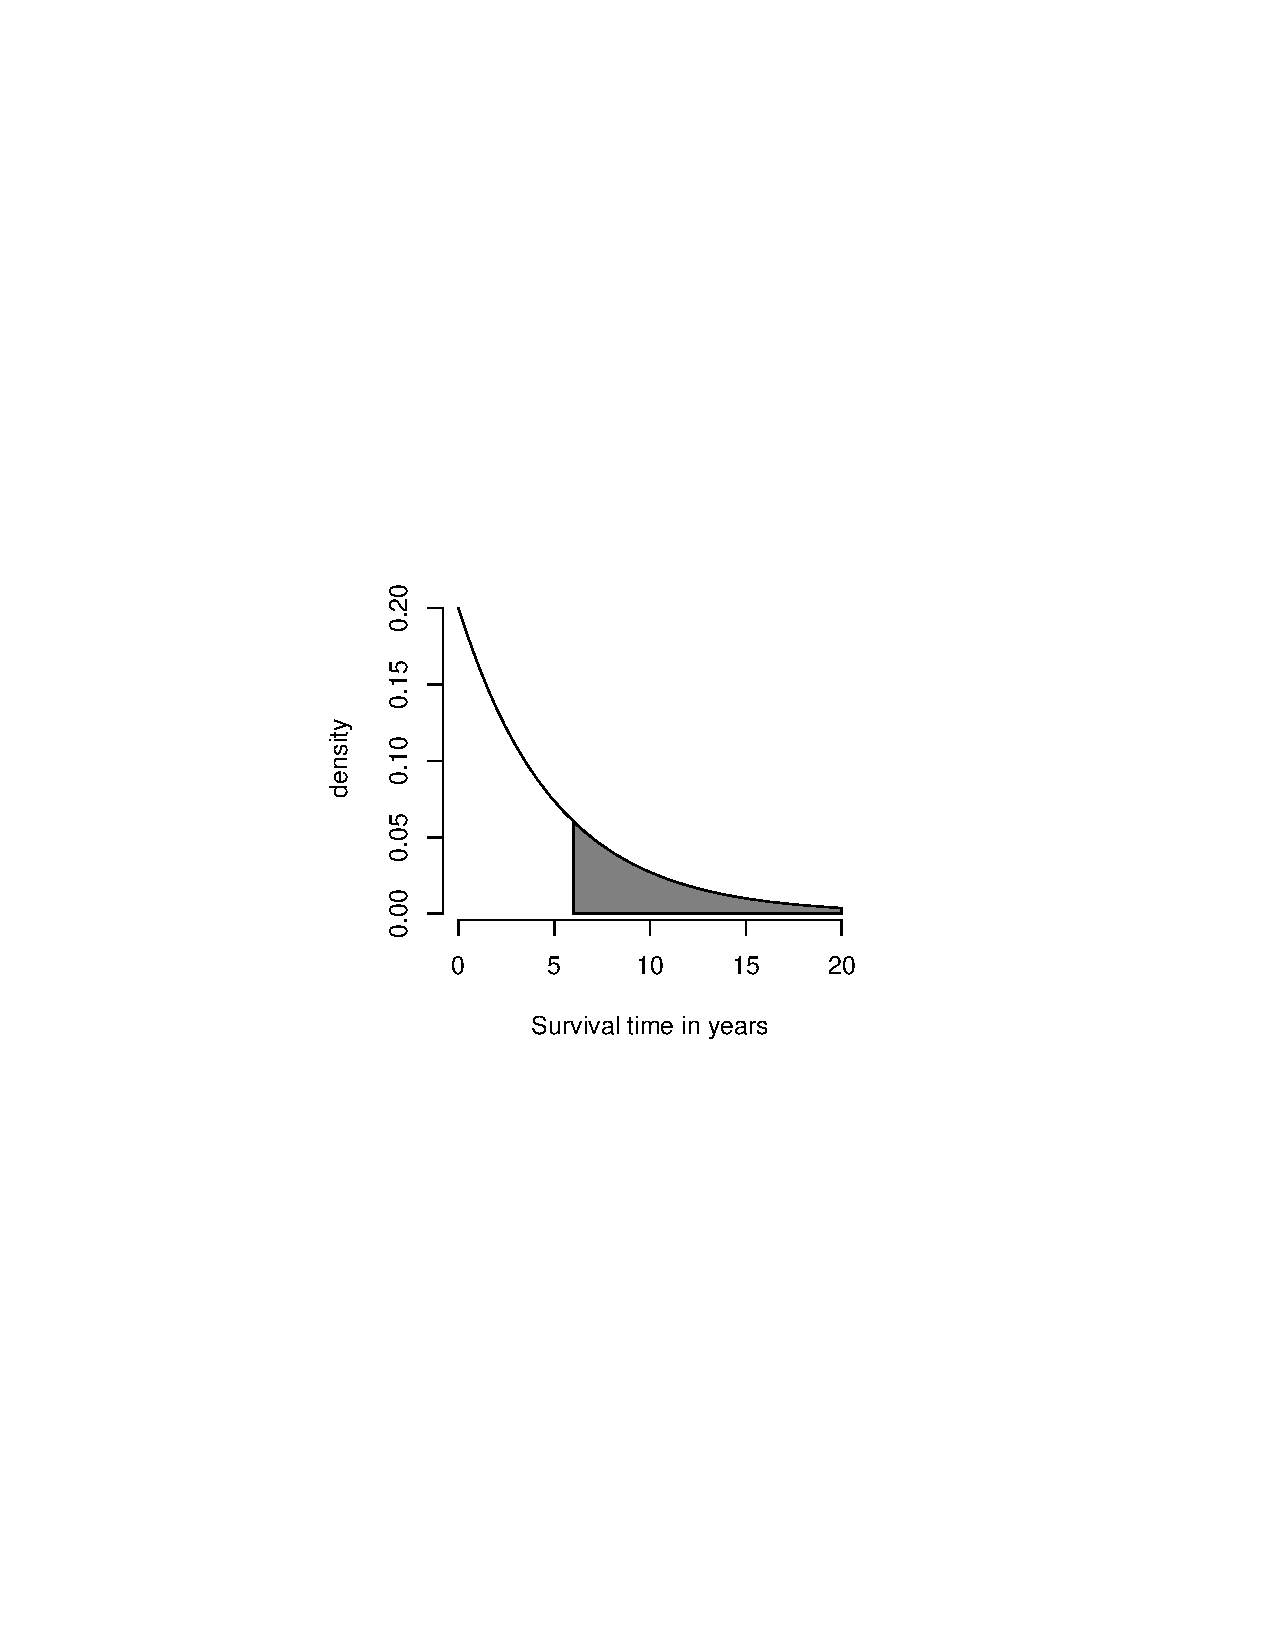
\includegraphics[width=3.5in]{exponential.pdf}
\end{frame}

\section{CDFs, survival functions and quantiles}
\begin{frame}
\frametitle{CDF and survival function}
\begin{itemize}
\item The {\bf cumulative distribution function} (CDF) of a random variable $X$
is defined as the function 
$$
F(x) = P(X \leq x)
$$
\item This definition applies regardless of whether $X$ is discrete or continuous.
\item The {\bf survival function} of a random variable $X$ is defined as
$$
S(x) = P(X > x)
$$
\item Notice that $S(x) = 1 - F(x)$
\item For continuous random variables, the PDF is the derivative of the CDF
\end{itemize}
\end{frame}

\begin{frame}
\frametitle{Example continued}
   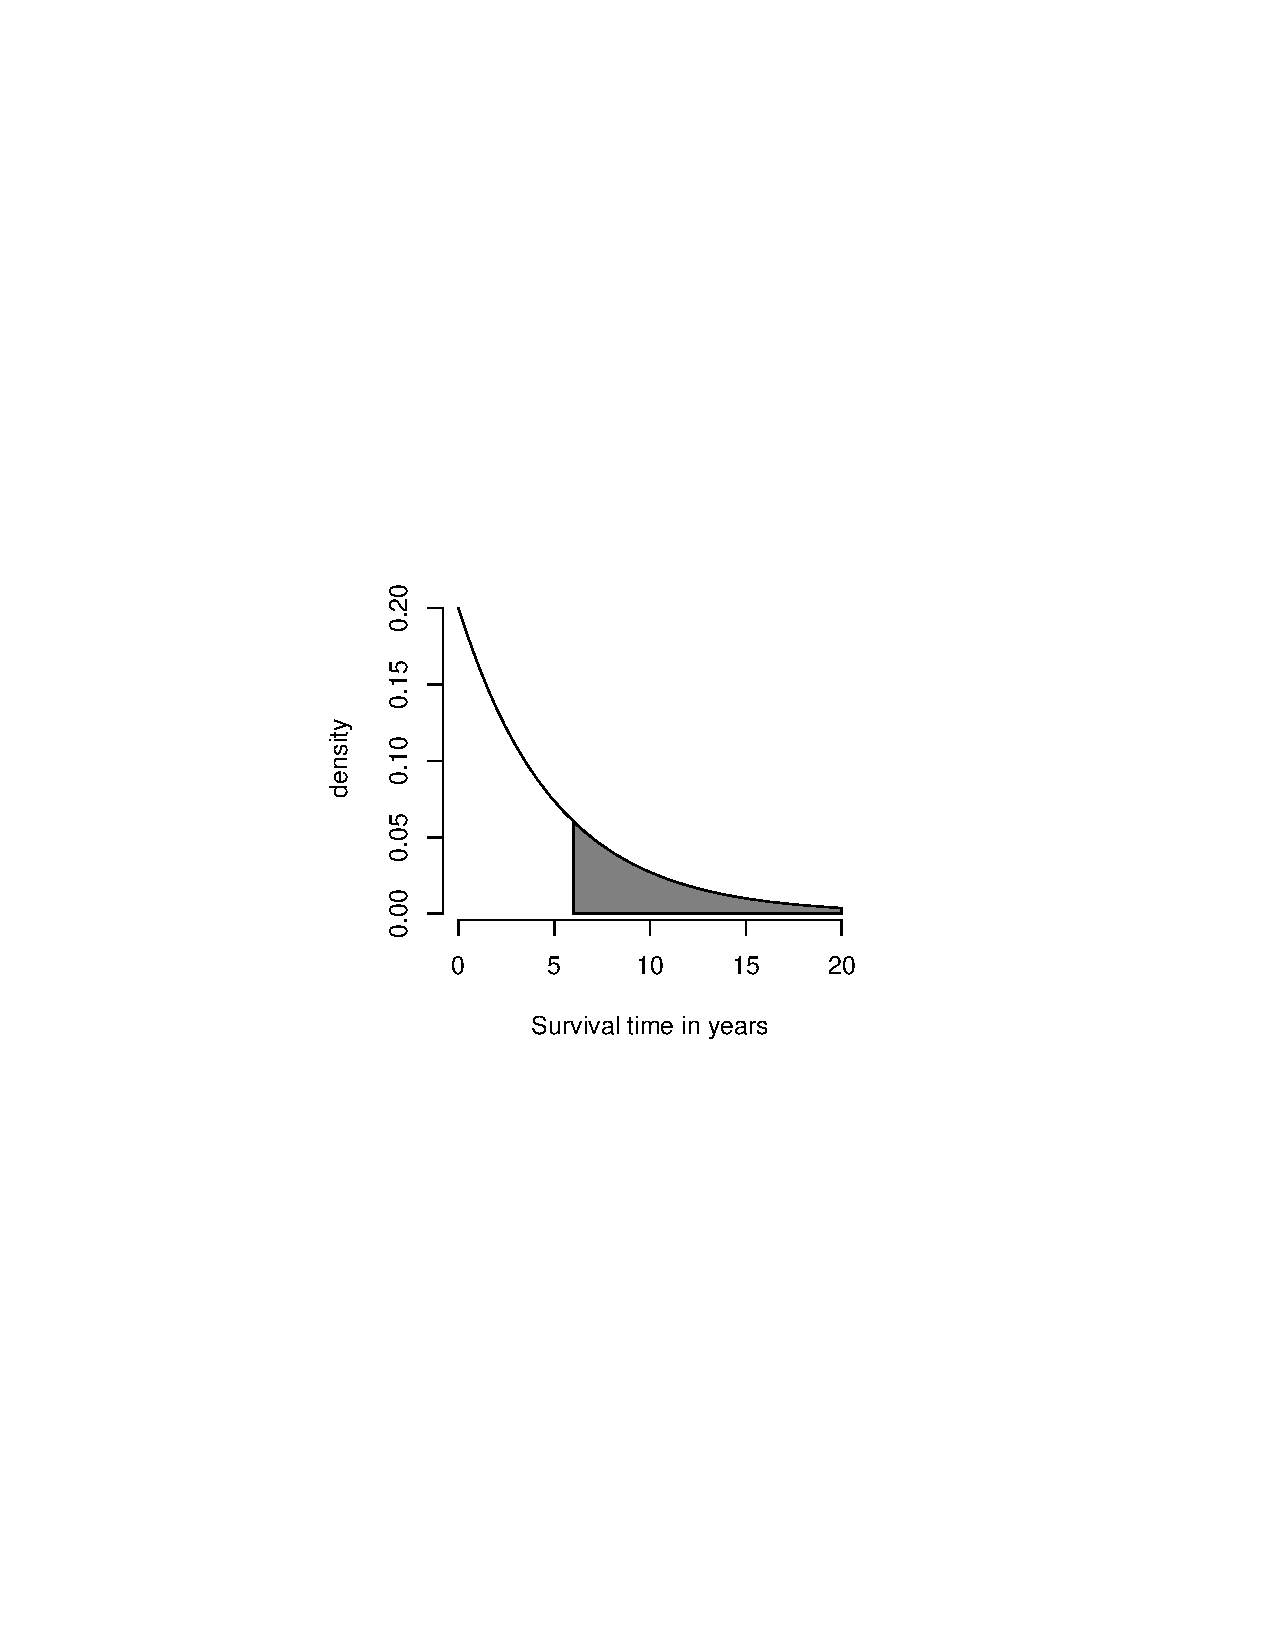
\includegraphics[width=3.5in]{exponential.pdf}
\end{frame}

\begin{frame}
\frametitle{Example}
What are the survival function and CDF from the exponential density considered before?
\end{frame}

\begin{frame}
\frametitle{Example}
What are the survival function and CDF from the exponential density considered before?
$$
S(x) = \int_x^\infty  \frac{e^{-t/5}}{5}dt =  \left. -e^{-t/5} \right|_{x}^\infty = e^{-x/5}
$$
hence we know that
$$
F(x) = 1 - S(x) = 1 - e^{-x/5}
$$
Notice that we can recover the PDF by
$$
f(x) = F'(x) = \frac{d}{dx} (1 -  e^{-x/5}) = e^{-x/5}/5
$$
\end{frame}


\begin{frame}
\frametitle{Quantiles}
\begin{itemize}
\item The  {\bf $\alpha^{th}$quantile} of a distribution with distribution function 
$F$ is the point $x_\alpha$ so that
$$
F(x_\alpha) = \alpha
$$
\item A {\bf percentile} is simply a quantile with $\alpha$ expressed as a percent
\item The {\bf median} is the $50^{th}$ percentile
\end{itemize}
\end{frame}

\begin{frame}
\frametitle{Example continued}
   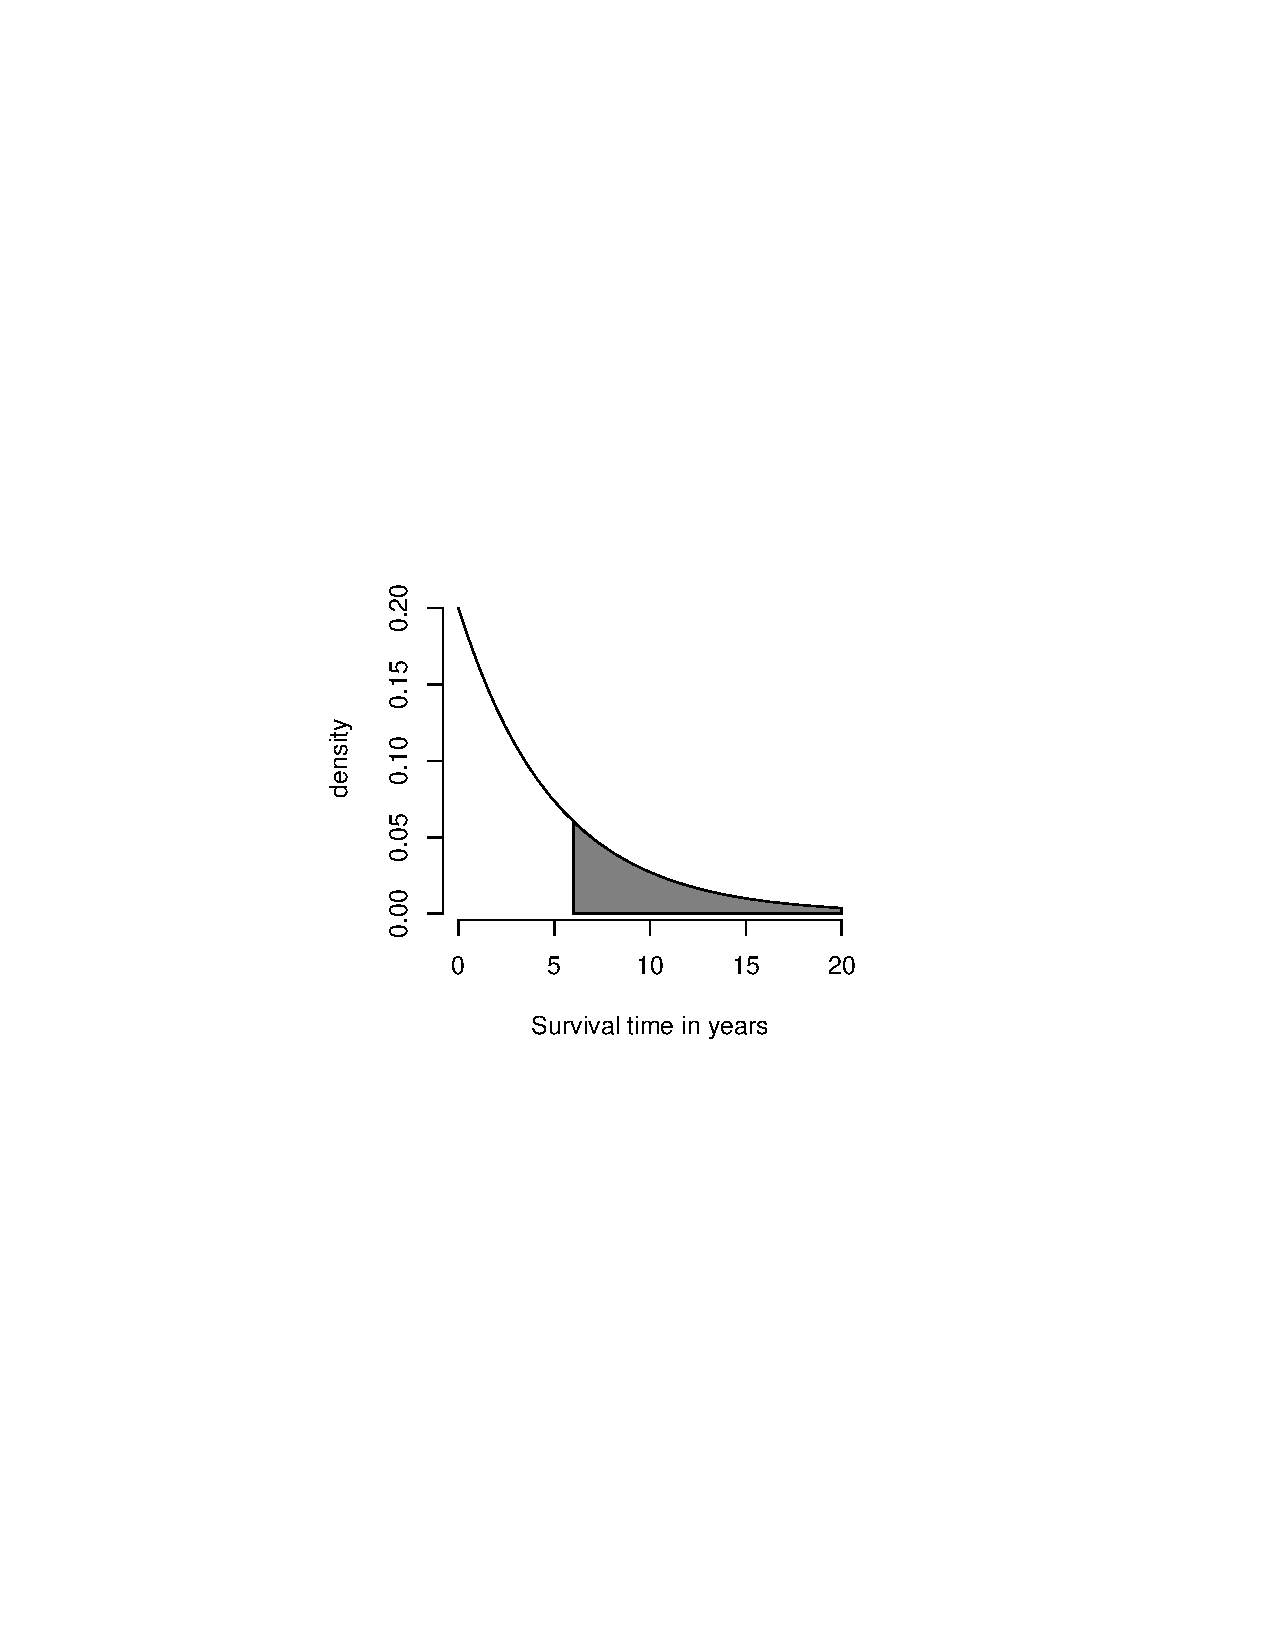
\includegraphics[width=3.5in]{exponential.pdf}
\end{frame}


\begin{frame}
\frametitle{Example}
\begin{itemize}
\item  What is the $25^{th}$ percentile of the exponential survival distribution considered before?
\end{itemize}
\end{frame}

\begin{frame}
\frametitle{Example}
\begin{itemize}
\item  What is the $25^{th}$ percentile of the exponential survival distribution considered before?
\item We want to solve (for $x$)
\begin{eqnarray*}
.25 & = & F(x) \\  
    & = & 1 - e^{-x/5}
\end{eqnarray*}
resulting in the solution $x = -\log(.75) \times 5 \approx 1.44$
\item Therefore, 25\% of the
subjects from this population live less than 1.44 years
\item R can approximate exponential quantiles for you \\
\texttt{qexp(.25, 1/5)}
\end{itemize}
\end{frame}


\section{Summary}
\begin{frame}
\frametitle{Probability models}
\begin{itemize}
\item You might be wondering at this point ``I've heard of a median before, it didn't require integration. Where's the data?''
\item We're referring to are {\bf population quantities}. Therefore, the median being
	discussed is the {\bf population median}.
\item A probability model connects the data to the population using assumptions.
\item Therefore the median we're discussing is the {\bf estimand}, the sample median will be the {\bf estimator}
\end{itemize}
\end{frame}

\end{document}

